\documentclass[10pt]{beamer}\usepackage[]{graphicx}\usepackage[]{color}
%% maxwidth is the original width if it is less than linewidth
%% otherwise use linewidth (to make sure the graphics do not exceed the margin)
\makeatletter
\def\maxwidth{ %
  \ifdim\Gin@nat@width>\linewidth
    \linewidth
  \else
    \Gin@nat@width
  \fi
}
\makeatother

\definecolor{fgcolor}{rgb}{0.345, 0.345, 0.345}
\newcommand{\hlnum}[1]{\textcolor[rgb]{0.686,0.059,0.569}{#1}}%
\newcommand{\hlstr}[1]{\textcolor[rgb]{0.192,0.494,0.8}{#1}}%
\newcommand{\hlcom}[1]{\textcolor[rgb]{0.678,0.584,0.686}{\textit{#1}}}%
\newcommand{\hlopt}[1]{\textcolor[rgb]{0,0,0}{#1}}%
\newcommand{\hlstd}[1]{\textcolor[rgb]{0.345,0.345,0.345}{#1}}%
\newcommand{\hlkwa}[1]{\textcolor[rgb]{0.161,0.373,0.58}{\textbf{#1}}}%
\newcommand{\hlkwb}[1]{\textcolor[rgb]{0.69,0.353,0.396}{#1}}%
\newcommand{\hlkwc}[1]{\textcolor[rgb]{0.333,0.667,0.333}{#1}}%
\newcommand{\hlkwd}[1]{\textcolor[rgb]{0.737,0.353,0.396}{\textbf{#1}}}%
\let\hlipl\hlkwb

\usepackage{framed}
\makeatletter
\newenvironment{kframe}{%
 \def\at@end@of@kframe{}%
 \ifinner\ifhmode%
  \def\at@end@of@kframe{\end{minipage}}%
  \begin{minipage}{\columnwidth}%
 \fi\fi%
 \def\FrameCommand##1{\hskip\@totalleftmargin \hskip-\fboxsep
 \colorbox{shadecolor}{##1}\hskip-\fboxsep
     % There is no \\@totalrightmargin, so:
     \hskip-\linewidth \hskip-\@totalleftmargin \hskip\columnwidth}%
 \MakeFramed {\advance\hsize-\width
   \@totalleftmargin\z@ \linewidth\hsize
   \@setminipage}}%
 {\par\unskip\endMakeFramed%
 \at@end@of@kframe}
\makeatother

\definecolor{shadecolor}{rgb}{.97, .97, .97}
\definecolor{messagecolor}{rgb}{0, 0, 0}
\definecolor{warningcolor}{rgb}{1, 0, 1}
\definecolor{errorcolor}{rgb}{1, 0, 0}
\newenvironment{knitrout}{}{} % an empty environment to be redefined in TeX

\usepackage{alltt}
\usetheme{metropolis}           % Use metropolis theme

\usepackage{graphicx}

\DeclareGraphicsExtensions{.pdf,.jpeg,.jpg,.png}

\usepackage{subcaption}
\usepackage{amsmath}

\usepackage{tikz}
\usetikzlibrary{bayesnet}
\usepackage{pgfplots}
\pgfplotsset{compat=1.13}

\usepackage[framemethod=TikZ, xcolor=RGB]{mdframed}
\definecolor{mydarkblue}{rgb}{0,.06,.5}
\definecolor{mydarkred}{rgb}{.5,0,.1}
\definecolor{myroyalblue}{rgb}{0,.1,.8}
\mdfdefinestyle{MyFrame}{%
    linecolor=mydarkblue,
    outerlinewidth=0.5pt,
    roundcorner=2pt,
    innertopmargin=2pt,
    innerbottommargin=2pt,
    innerrightmargin=2pt,
    innerleftmargin=2pt,
    backgroundcolor=blue!10}

\newcommand{\Rbb}{\mathbb{R}}
\newcommand{\Expect}{\mathbb{E}}
\newcommand{\Expecthat}{\hat{\mathbb{E}}}
\newcommand{\Var}{\text{Var}}
\newcommand{\Cov}{\text{Cov}}
\newcommand{\vbfamily}{\mathcal{Q}}
\newcommand{\etaopt}{\eta^{*}}
\newcommand{\etazopt}{\eta_z^{*}}
\newcommand{\etathetaopt}{\eta_\theta^{*}}
%\newcommand{\qopt}{q^{*}}
\newcommand{\targethat}{\hat{g}}
\newcommand{\QExpect}
{\Expect_{q\left(\theta, z \vert \eta_\theta, \etazopt(\eta_\theta)\right)}}
\newcommand{\atzero}{\Big\rvert_{\eta_\theta = \etathetaopt, \epsilon = 0}}
\newcommand{\etathetalin}{\eta_\theta^{LIN}}
\DeclareMathOperator*{\argmin}{arg\,min}





\title{Evaluating Sensitivity to the Stick Breaking Prior in
Bayesian Nonparametrics}
\date{December 7, 2018}
\author{Runjing (Bryan) Liu}
\institute{University of California, Berkeley}

\setbeamertemplate{Collaborators}[none]
\IfFileExists{upquote.sty}{\usepackage{upquote}}{}
\begin{document}
\maketitle

\begin{frame}{Collaborators}
  	\vspace{1em}
  	\begin{figure}
  		\begin{subfigure}{.4\textwidth}
  			\centering
  			
\includegraphics[height=2cm]{collaborators/bryan}
        \captionsetup{justification=centering}
  			\caption*{Runjing (Bryan) Liu \\ UC Berkeley}
  		\end{subfigure}%
  		\begin{subfigure}{.4\textwidth}
  			\centering
  			
\includegraphics[height=2cm]{collaborators/ryan}
  			\caption*{Ryan Giordano \\ UC Berkeley}
  		\end{subfigure}\\ \vspace{0.11in}
      \begin{subfigure}{.4\textwidth}
  			\centering
  			
\includegraphics[height=2cm]{collaborators/mike}
  			\caption*{Michael I.\ Jordan \\ UC Berkeley}
  		\end{subfigure}%
  		\begin{subfigure}{.4\textwidth}
  			\centering
  			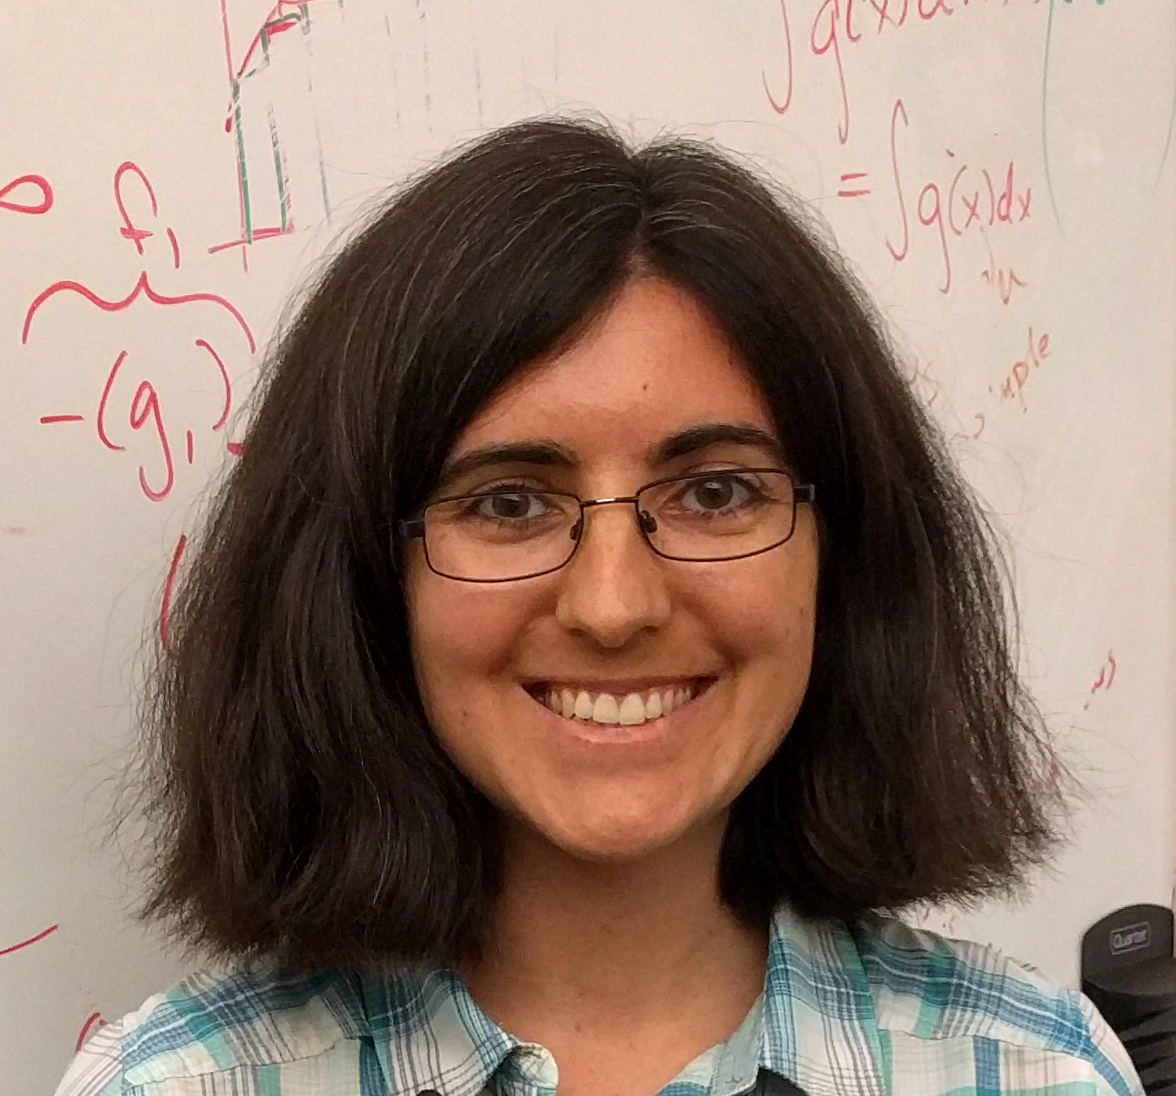
\includegraphics[height=2cm]{collaborators/tamara}
  			\caption*{Tamara Broderick \\ MIT}
  		\end{subfigure}\\
  	\end{figure}

\end{frame}

\begin{frame}{Question of Interest}

We are interested in inferring the number of clusters in a dataset.

\pause
\begin{figure}[!h]
\centering
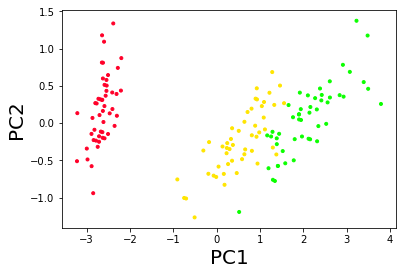
\includegraphics[width = 0.5\textwidth]{./images/iris_data.png}
%\caption{The iris data projected onto the first two principal components. Color corresponds to the true iris species. }

\setlength{\textfloatsep}{-10pt}
\end{figure}
\pause

A Bayesian nonparametric (BNP) model makes inferring the number of clusters amenable to
Bayesian inference.

\pause

\textbf{Question}: \textbf{how sensitive are the resulting
inferences on cluster cardinality to BNP model choices}?

\end{frame}

\begin{frame}{Outline}
   \tableofcontents
\end{frame}

\section{The BNP Model}

\begin{frame}{The BNP Model}
We model the prior on the cluster memberships $z_n$ using a
a stick breaking representation of a BNP Dirichlet process prior.
\vspace{-0.1in}
\begin{figure}[!h]
\centering
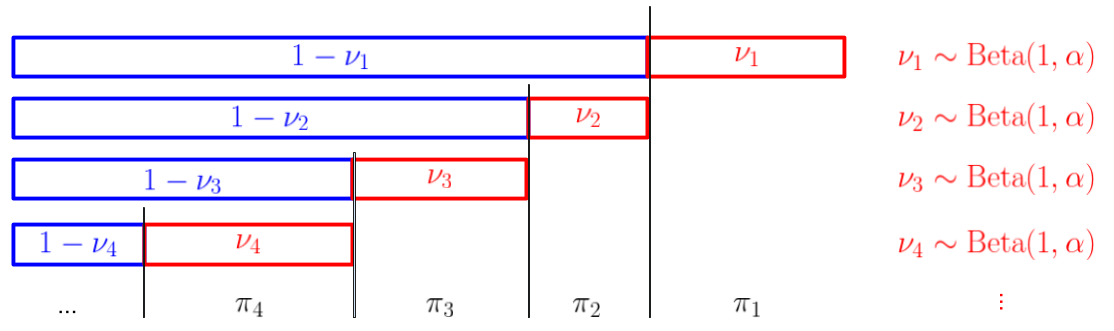
\includegraphics[width = 0.95\textwidth]{./figures/DP_stick_breaking.png}
\end{figure}
\vspace{-0.1in}
The prior on the cluster proportions $\pi_1, \pi_2, ..., $ are given by
%
\begin{align*}
\nu_k \vert \alpha &\overset{\text{iid}}{\sim} \text{Beta}\left(1, \alpha \right)\quad k = 1, 2, ..., \infty \\
\pi_k | \nu &:= \nu_k \prod_{j=1}^{k-1} (1 - \nu_j) \quad k = 1, 2, ..., \infty
\end{align*}
% The stick-breaking proportions are drawn from a beta distribution, and the weights are then defined :
% \begin{align*}
% \nu_k \vert \alpha \overset{\text{iid}}{\sim} \text{Beta}\left(1, \alpha \right) \quad k = 1, 2, ..., \infty
% \end{align*}
% The cluster proportions are defined:
% \begin{align*}
% \pi_k | \nu := \nu_k \prod_{j=1}^{k-1} (1 - \nu_j) \quad k = 1, 2, ..., \infty
% \end{align*}
%
\vspace{-0.1in}\pause 
%
\begin{mdframed}[style=MyFrame]
\begin{center}
{\bf What makes this stick-breaking prior a reasonable one?}
\end{center}
\end{mdframed}

\end{frame}

\begin{frame}{The BNP Model}
The cluster belongings are then drawn
\begin{align*}
  z_n \vert \pi \overset{\text{iid}}{\sim} \mathrm{Categorical}(\pi)
  \quad n = 1, 2, ..., N
\end{align*}
%
And the data $y_n$ are drawn,
\begin{align*}
	y_n | z_n, \mu, \Sigma \sim
        \mathcal{N}\left(
            y_n \Big\vert
                \sum_{k=1}^\infty \mathbb{I}\{z_n = k\} \mu_k \;,
              \; \sum_{k=1}^\infty \mathbb{I}\{z_n = k\} \Sigma_k\right),
	\quad n = 1, ..., N.
\end{align*}
%
With conjugate priors for $\mu$ and $\Sigma$.

\end{frame}

\section{The Variational Approximation}

\begin{frame}{The Variational Approximation}
We use take a mean-field variational distribution where the 
\begin{itemize}
\item stick-breaking proportions $\nu_k$ are logitnormal; 
\item the cluster centroids $\mu_k$ and cluster covariances $\Sigma_k$ are point masses; 
\item and the cluster belongings $z_n$ are categorical. 
\end{itemize}
\end{frame}

% \begin{align*}
%   \mathcal{Q} := \Big\{ q:
%   q(\nu, \mu, \Sigma, z) &=
%   \left(\prod_{k=1}^{K}q\left(\nu_{k}\right)\delta\left(\mu_{k}\right)
%       \delta\left(\Sigma_{k}\right)\right)
%       \left(\prod_{n=1}^{N}q\left(z_{n}\right) \right)\textrm{, where } \\
%   q\left(\nu_{k}\right) &= \mathrm{Lognormal}\left(\nu_k\right) \textrm{ and }
%   q\left(z_n\right) = \mathrm{Categorical}\left(z_n\right)
%   \Big\}.
% \end{align*}

\begin{frame}{The Variational Approximation}

Define:

- $\eta_\theta$: the variational parameters for the global parameters
(the stick-breaking proportions, the cluster centroids, the cluster covariances).

- $\eta_z$: the variational parameters for the categorical distributions on the
cluster belongings $z$.

Note that by choosing a conditionally conjugate model for the cluster belongings,
for a given $\eta_\theta$ we can solve in closed form the optimal $\eta_z$.

\pause

Our objective is then
\begin{align*}
  \argmin_{\eta_\theta} KL\left(
      q(\theta, z \vert \eta_\theta, \eta_z^*(\eta_\theta) \big\| p(\theta, z | y)
      \right)
\end{align*}
%
{\bf All posterior quantities are then functions of $\eta_\theta$. }

\end{frame}

\begin{frame}{The Posterior Quantity of Interest}

We are interested in discovering how many clusters are present. 

\pause
We can ask: 
\begin{enumerate}[(1)]
\item Under a BNP model, how many distinct components exist in the world? 
\pause
\item How many clusters would we expect to be present in a {\bf new} dataset of particular size?
\pause
\item How many clusters are present in the {\bf current} dataset?
\end{enumerate}

\end{frame}

\begin{frame}{The Posterior Quantity of Interest}
Question (2) asks for a {\bf predictive} quantity: 
\begin{align*}
g_{pred}(\etathetaopt) &:=
\Expect_{q(\nu \vert \etathetaopt)} \left[\#\{\text{clusters in new data set of size $N$}\} \right]  \\
&=
\Expect_{q(\nu \vert \etathetaopt)} \left[\sum_{k=1}^K \left(1 - (1 - \pi_k)^{N}\right)\right].
% g_{t, pred}(\etathetaopt) &:=
% \Expect_{q(\nu \vert \etathetaopt)} \left[\#\{\text{clusters in new data set with at least $t$ data points}\} \right]  \\
% &=
% \Expect_{q(\nu \vert \etathetaopt)} \left[\sum_{k=1}^K \left(1 - \sum_{i = 0}^t {n\choose i}
% \pi_k^{i} (1 - \pi_k)^{n - i}\right)\right].
\end{align*}
%
\pause 
%
Question (3) asks for an {\bf in-sample} quantity: 
\begin{align*}
g(\etathetaopt) &:=
\Expect_{q(z \vert \etazopt(\etathetaopt))} \left[ \#\{\text{distinct clusters}\} \right]  \\
&=
\Expect_{q(z \vert \etazopt(\etathetaopt))} \left[
    \sum_{k=1}^K \left(1 - \prod_{n=1}^N \mathbb{I}\{z_n \ne k\} \right)
    \right]
% g_t(\etathetaopt) &:=
% \Expect_{q(z \vert \etazopt(\etathetaopt))} \left[ \#\{\text{clusters with at least $t$ data points}\} \right]  \\
% &=
% \Expect_{q(z \vert \etazopt(\etathetaopt))} \left[
%     \sum_{k=1}^K \mathbb{I}\left\{\left(\sum_{n=1}^N \mathbb{I}\{z_n = k\} \right) \geq t \right\}\right].
\end{align*}
%
\pause\vspace{-0.1in}
%
\begin{mdframed}[style=MyFrame]
\begin{center}
{\bf How do these quantities vary as the BNP prior varies? }
\end{center}
\end{mdframed}

\end{frame}


\section{Hyperparameter Sensitivity}

\begin{frame}{Hyperparameter Sensitivity}

Let $\epsilon$ be a real-valued hyperparameter for the stick-breaking distribution
(e.\ g., this could be the $\alpha$ concentration parameter, or it could parameterize a functional shape).

\pause

The expected number of clusters present in the {\itshape current} iris dataset is a composition of the functions,
\begin{align*}
  \epsilon \mapsto
  \etathetaopt(\epsilon) \mapsto
  \etazopt\left(\etathetaopt\right) \mapsto
  \Expect_{q(z | \etazopt)} \left[ \#\{\text{distinct clusters}\} \right].
\end{align*}

\pause

Similarly for the predictive quantity, the expected number of clusters present in a {\itshape new} dataset:
\begin{align*}
  \epsilon \mapsto
  \etathetaopt(\epsilon) \mapsto
  \Expect_{q(\nu \vert \etathetaopt)}
  \left[\#\{\substack{\text{distinct clusters}\\\text{in new dataset}}\} \right].
\end{align*}


\end{frame}

\begin{frame}{Hyperparameter Sensitivity}

We approximate the dependence of $\etathetaopt$ on $\epsilon$ with a first-order
Taylor expansion:

\begin{align*}
  \etathetaopt(\epsilon)  &\approx  \etathetaopt(0) +
  \frac{d \etathetaopt(\epsilon)}{d\epsilon^T}\Big|_{\epsilon=0} \epsilon
\end{align*}
\end{frame}


\begin{frame}{Hyperparameter Sensitivity}
We compute the derivative following Giordano et al. 2018:
\begin{align*}
\frac{d \etathetaopt(\epsilon)}{d\epsilon^T}\Big|_{\epsilon=0} = H^{-1}f_\eta
\end{align*}
where
\begin{align*}
  H &:= \frac{\partial^2 KL(\eta_\theta, \epsilon) }{
      \partial \eta_\theta \partial \eta_\theta^T}
      \atzero
\\
  f_\eta &:= \frac{\partial^2
      \QExpect \left[ \log p\left(y, \theta, z \vert \epsilon \right) \right]}{\partial \eta_\theta \partial \epsilon}
      \atzero.
\end{align*}

These computations are done efficiently using automatic differentiation (Maclaurin et al. 2015). 

\end{frame}

\section{Results}

\begin{frame}{Results}

We use BNP to infer the number of species in iris dataset (Anderson 1936). 

\begin{figure}[!h]
\centering
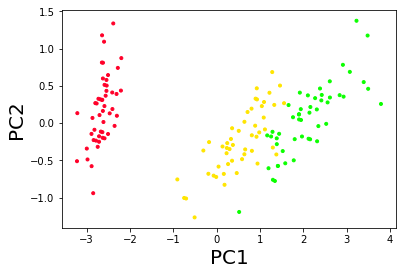
\includegraphics[width = 0.6\textwidth]{./images/iris_data.png}

\caption{The iris data projected onto the first two principal components. Color corresponds to the true iris species. }

\setlength{\textfloatsep}{-10pt}
\end{figure}

\end{frame}

\begin{frame}{Results: parametric sensitivity}

Suppose we wish to evaluate the sensitivity to the DP concentration parameter $\alpha$.

\pause 

Let $\alpha_0$ be a base value of $\alpha$ at which we optimize for
$\etaopt$. We can apply the previous formula by taking $\epsilon = \alpha - \alpha_0$, and setting 
\begin{align*}
f^\alpha_\eta := \frac{\partial^2
    \QExpect
        \left[ \log p\left(\nu \vert \alpha \right) \right]}
{ \partial \eta_\theta \partial \alpha^T }
    \Big\rvert_{\eta_\theta = \etathetaopt, \alpha = \alpha_0},
\end{align*}

\end{frame}

\begin{frame}{Results: parametric sensitivity}

\begin{figure}
\centering
\begin{knitrout}
\definecolor{shadecolor}{rgb}{0.969, 0.969, 0.969}\color{fgcolor}

{\centering 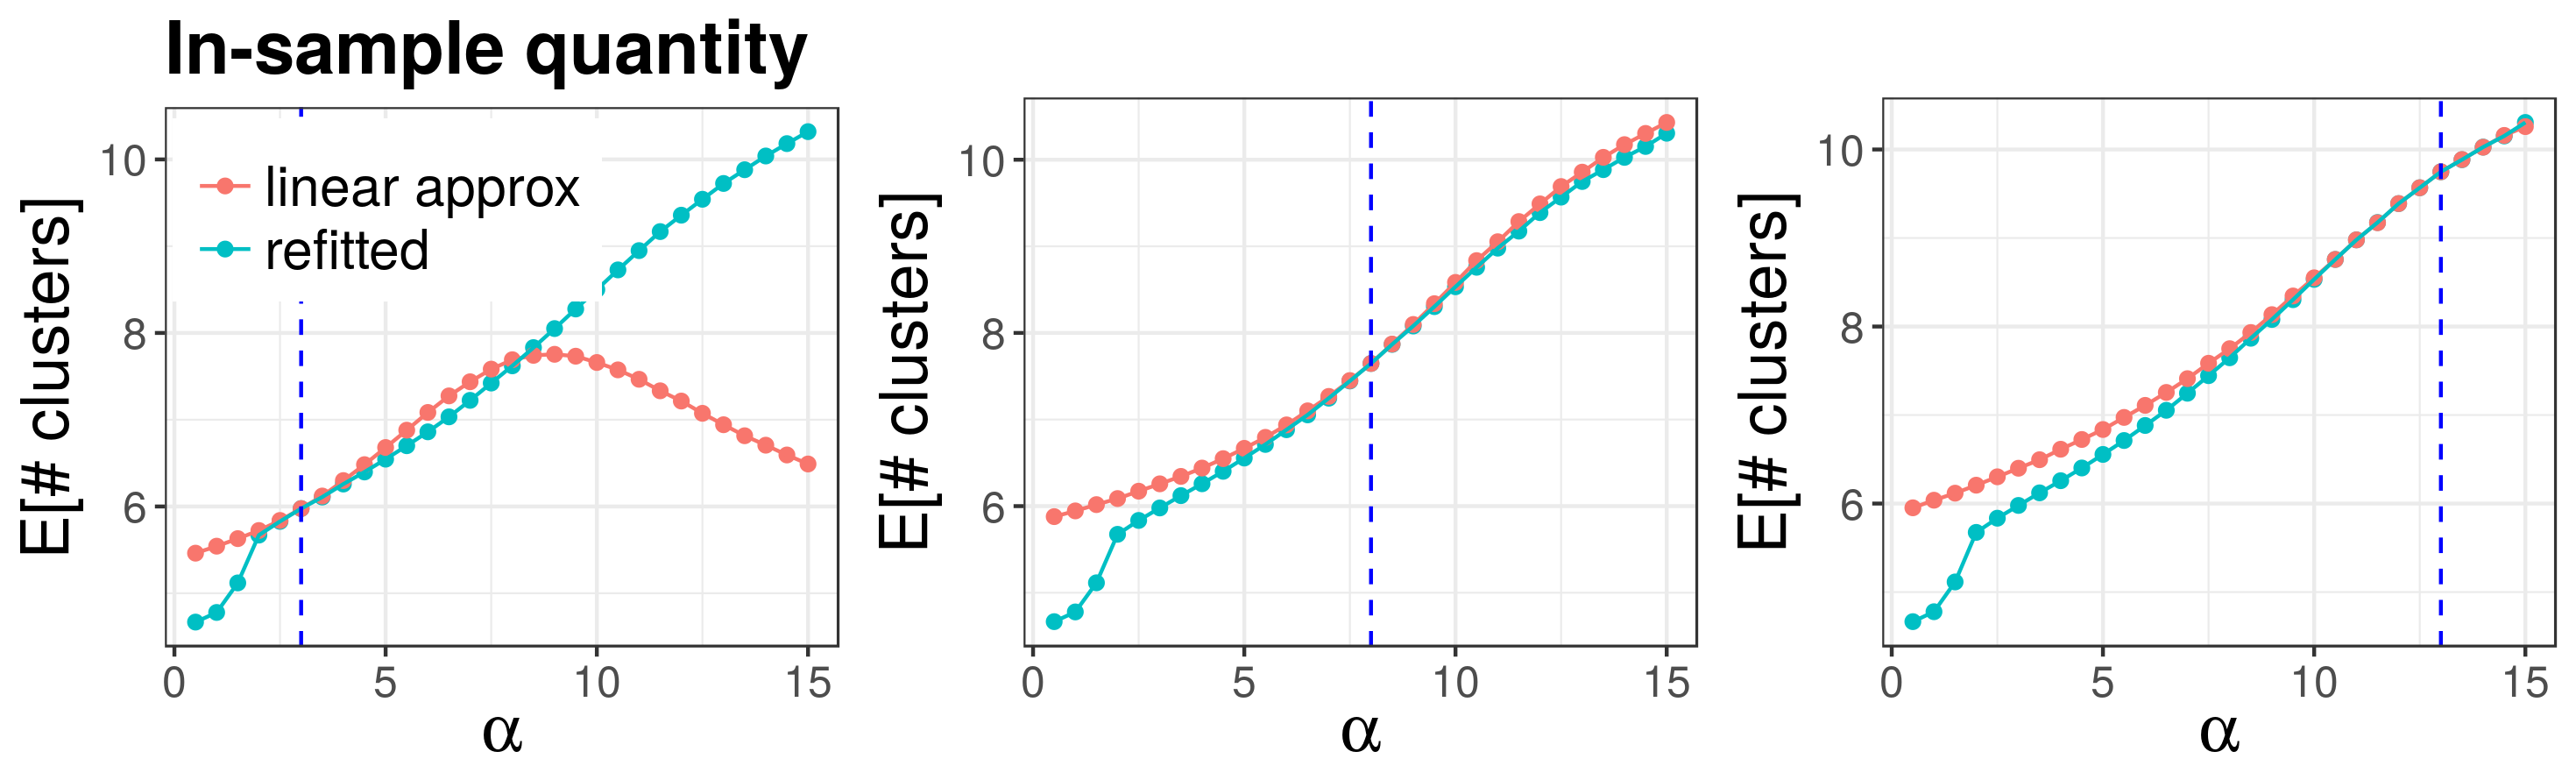
\includegraphics[width=0.98\linewidth,height=0.294\linewidth]{figure/param_sens_plot_thresh_0-1} 

}



\end{knitrout}
\begin{knitrout}
\definecolor{shadecolor}{rgb}{0.969, 0.969, 0.969}\color{fgcolor}

{\centering 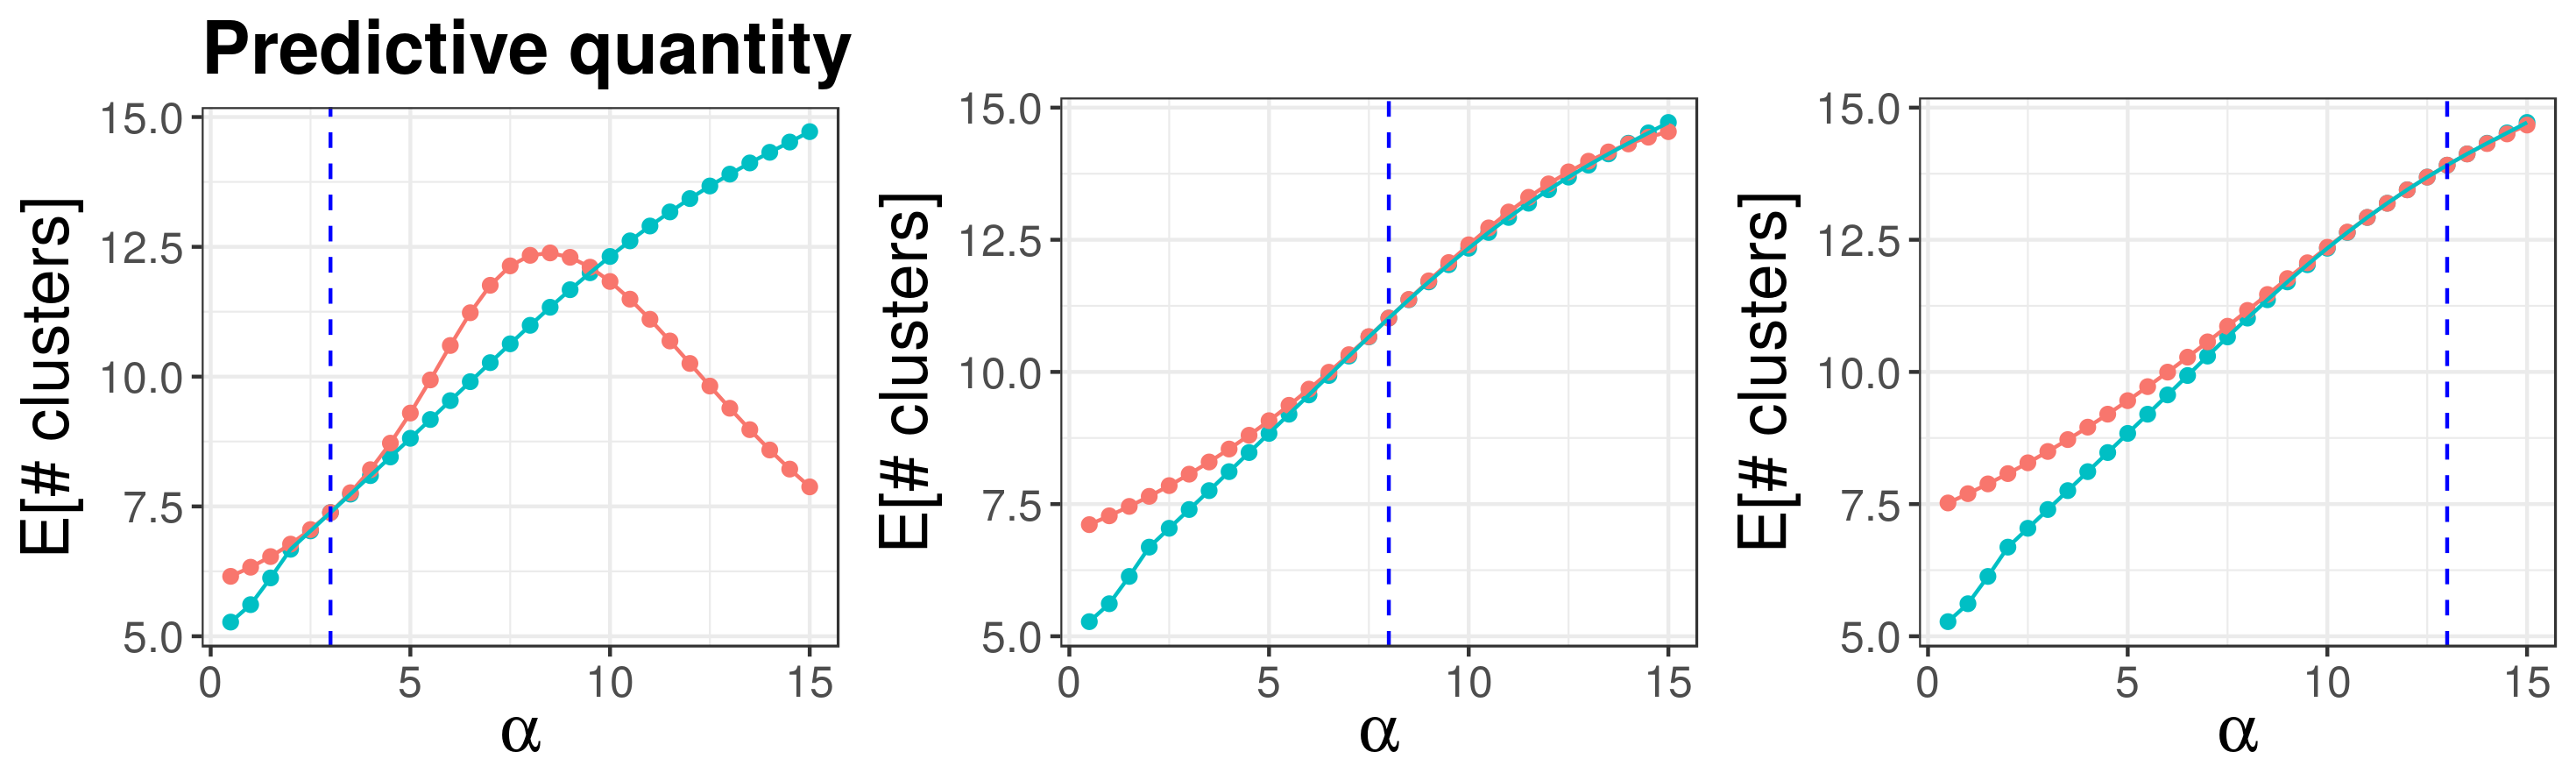
\includegraphics[width=0.98\linewidth,height=0.294\linewidth]{figure/param_sens_plot_thresh_0b-1} 

}



\end{knitrout}
\caption{Comparison of in-sample (top) and predictive (bottom) expected number of clusters computed by re-optimizing versus the linear approximation. 
The blue vertical line indicates the location of $\alpha_0$}
\end{figure}

\end{frame}

\begin{frame}{Results: functional perturbation}
Now consider a multiplicative perturbation $\phi$ to
the original beta distribution $p_0$ for the stick-breaking proportions:
%
\begin{align*}
\label{eq:expon_perturb}
	p_c(\nu_k \vert \delta, \phi) :=
  \frac{p_{0}(\nu_k)\phi(\nu_k)^\delta}
       {\int_0^1 p_0(\nu_k')\phi(\nu')^\delta d\nu_k'}.
\end{align*}

\pause 

For a fixed $\phi$, we can use our approximation by taking
$\epsilon = \delta$ and
%
\begin{align*}
f^{\delta,\phi}_\eta &:=
\frac{\partial^2
    \QExpect \left[ \sum_{k=1}^K \log p_c(\nu_k \vert \delta, \phi) \right]}
{\partial \eta_\theta \partial \delta}
    \Big\rvert_{\eta_\theta = \etathetaopt, \delta = 0} \\
    &=
\frac{\partial
    \QExpect \left[ \sum_{k=1}^K  \log\phi(\nu_k) \right]}
{\partial \eta_\theta}
    \Big\rvert_{\eta_\theta = \etathetaopt}.
\end{align*}

\end{frame}


\begin{frame}{Results: functional perturbation}
\begin{figure}
\centering

\begin{knitrout}
\definecolor{shadecolor}{rgb}{0.969, 0.969, 0.969}\color{fgcolor}

{\centering 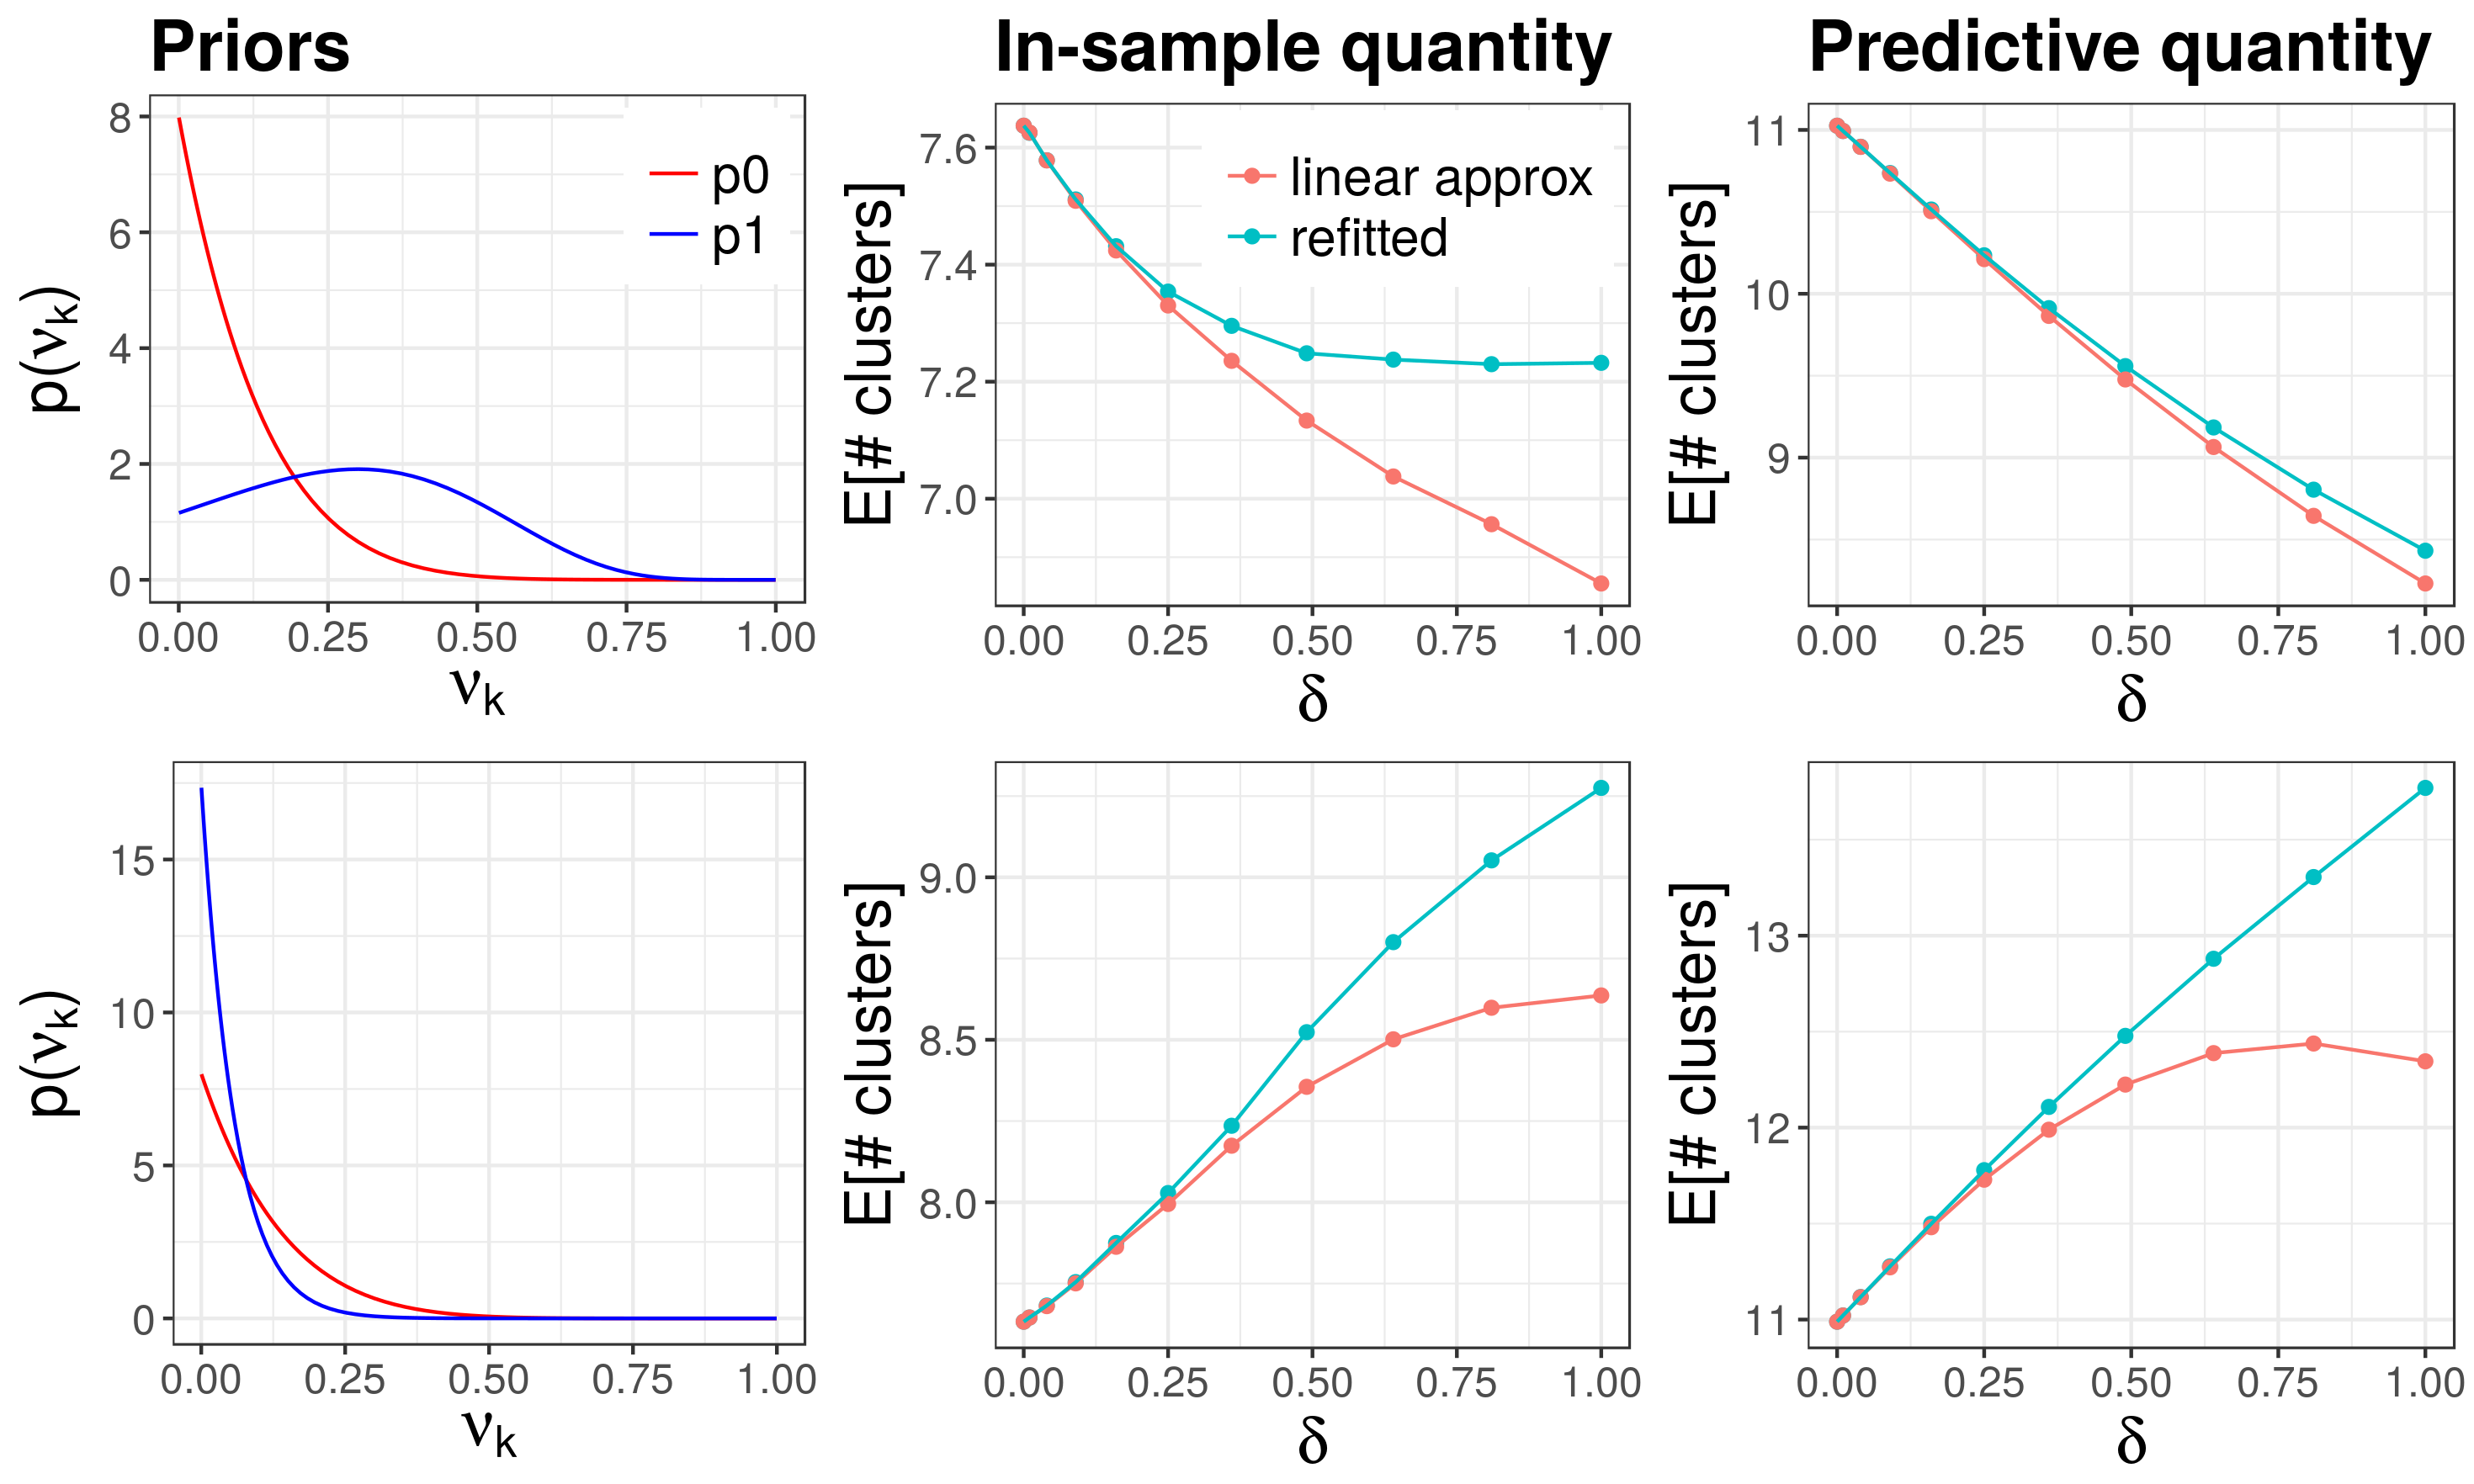
\includegraphics[width=0.98\linewidth,height=0.588\linewidth]{figure/functional_sens_plot_thresh0-1} 

}



\end{knitrout}
\caption{The effect of prior perturbation on the expected number of distinct clusters. Left column: the original prior $p_0$ in red, the perturbed prior $p_c$, $\delta = 1$, in blue. Middle and right column: linearly approximated vs.
re-fitted expected number of clusters}
\end{figure}

\end{frame}

\begin{frame}{Summary}

\begin{itemize}

\item The linear approximation provides a fast and reasonable alternative to re-evaluating the full model after changing the BNP prior. 

\pause 

\item We applied the approximation to both parametric and functional perturbations to the stick-breaking prior.

\pause 

\item For the functional perturbation, we proposed to use multiplicative perturbations to improve linearity. 

\pause 

\item Furthermore, we approximated only the dependence of the global parameters on the prior parameter. We retained the non-linearity of the map from global parameters to posterior quantity.

\end{itemize}


\end{frame}

\begin{frame}

Thank you!

\end{frame}

\begin{frame}{References}

\begin{itemize}
\item E. Anderson. The species problem in iris. {\itshape Annals of the Missouri Botanical Garden}, 23(3):457–509, 1936.

\item R. Giordano, T. Broderick, and M. I. Jordan. Covariances, robustness, and variational Bayes. {\itshape Journal of Machine Learning Research}, 19(51):1–49, 2018.

\item D. Maclaurin, D. Duvenaud, and R. P. Adams. Autograd: Effortless gradients in numpy. {\itshape In International Conference on Machine Learning 2015 AutoML Workshop}, 2015.

\end{itemize}

\end{frame}


\end{document}
